\documentclass[a4paper]{article}

%% Language and font encodings
\usepackage[english]{babel}
\usepackage[utf8x]{inputenc}
\usepackage[T1]{fontenc}

%% Sets page size and margins
\usepackage[a4paper,top=3cm,bottom=2cm,left=3cm,right=3cm,marginparwidth=1.75cm]{geometry}

%% Useful packages
\usepackage{amsmath}
\usepackage{graphicx}
\usepackage[colorinlistoftodos]{todonotes}
\usepackage[colorlinks=true, allcolors=blue]{hyperref}
\usepackage{listings}
\usepackage{color} %red, green, blue, yellow, cyan, magenta, black, white
\definecolor{mygreen}{RGB}{28,172,0} % color values Red, Green, Blue
\definecolor{mylilas}{RGB}{170,55,241}

\title{An Overview of Sorting Algorithms\\MATH 3000 Final Project}
\author{Alec Graves\\Kennesaw State University}

\begin{document}
\lstset{language=Matlab,%
    %basicstyle=\color{red},
    breaklines=true,%
    morekeywords={matlab2tikz},
    keywordstyle=\color{blue},%
    morekeywords=[2]{1}, keywordstyle=[2]{\color{black}},
    identifierstyle=\color{black},%
    stringstyle=\color{mylilas},
    commentstyle=\color{mygreen},%
    showstringspaces=false,%without this there will be a symbol in the places where there is a space
    numbers=left,%
    numberstyle={\tiny \color{black}},% size of the numbers
    numbersep=9pt, % this defines how far the numbers are from the text
    emph=[1]{for,end,break},emphstyle=[1]\color{blue}, %some words to emphasise
    %emph=[2]{word1,word2}, emphstyle=[2]{style},    
}

\maketitle

\begin{abstract}
Sorting is a fundamental problem in computer science. It is often applied when there is a need to operate efficiently on a large set of data. Given the importance of sorting in modern computer science, it is paramount that one has available a relatively comprehensive resource covering the complexity, performance, and implementation of a variety of popular sorting algorithms. This paper provides such a resource.\end{abstract}

\section{Introduction}

Sorting, an important operation which forms the basis of many algorithms and solutions to problems in computer science, is a process which involves ordering unordered data. There are several popular algorithms which can be used for this task, and there are trade-offs for each one. Some algorithms which are faster operating on large sets of data will be slower operating on smaller sets. Some algorithms are faster but require much more memory. Some algorithms require fewer instructions to implement but are much slower.

This paper will address many of these trade-offs for several sorting algorithms, while providing implementation details and speed of execution. Data will be gathered using MATLAB r2018a so some interpreter wizardry may be occurring in the background. No steps have been taken to prevent interpreter optimizations besides avoiding built-in functions such as $min$ or $max$. The computer used in this work is a Microsoft Surface Pro 4 with 4GB of memory and an Intel Core i5-6300U CPU capable of operating at 2.4GHz. The full source for every example is included in this work. All source is available under the simple and permissive MIT license.
 

\section{Background}

\subsection{Importance of Sorting}

Sorting is a fundamental problem in computer science. Additionally, many problems that we face even today can be simplified or made faster using sorting. One example is using a sorting algorithm to pre-process data for an improved search time with methods such as binary search. Another example is efficiently finding the minimum, maximum, or median of a set of data by first sorting it. More examples of using sorting to make the solution to a problem include:

\begin{itemize}
\item \textbf{Element Uniqueness:} Are there repeats in a set of $n$ items?

\item{\textbf{Closest Pair:} How do you find the closest pair of items in a set of $n$ items?}

\item \textbf{Frequency Distribution:} Which element in a set of $n$ items occurs most frequently?

\item \textbf{Selection:} What is the $k^{th}$ largest item in the set?

\item \textbf{Convex Hulls:} Given n points in two dimensions, what is the polygon of the smallest area contains them all?
\end{itemize}

These problems can be more efficiently solved using sorting algorithms to pre-process data rather than operating on unsorted data directly. Additionally, much of computer science involves operating on unsorted data, and for this reason, sorting algorithms have the potential to improve the efficiency of solutions to many problems faced by computer scientists.

\subsection{Time Complexity}

Time complexity is a metric which deals with the limit of the time an algorithm takes as the length of its input increases. This metric, while giving a good overview of the limits of performance of an algorithm, is relatively flawed when it comes to actual application. One such limitation is performance on sets with very few elements. In these situations, complex algorithms may be much slower due to the overhead of processing many operations per element. Another limitation could be the number of instructions, which can become important when operating with on a system with limited memory or attempting to build circuits which execute the program. In these situations, simplicity of an algorithm could be much more important than the limit of time required as the size of the input increases. For this reason, time complexity will be analyzed along with the total number of operations given an input of size n. 

\subsection{Space Complexity}
Space complexity is a metric analyzing the limits of the space required to run an algorithm as the length of the input approaches a large number n. Like time complexity, this metric is flawed, not accounting for memory consumption of variables at smaller input lengths. For this reason, this paper’s analysis will focus on the memory consumption of variables used during execution as well as the limit of this number as the size of the input increases.

\subsection{MATLAB}
MATLAB is an interpreted language built with an emphasis on matrix operations. There are many parallels to C and BASIC languages in its syntax, but there are several key differences as well. In general, the syntax is simple enough to follow, and any confusing syntax can be understood with a few minutes of searching through MATLAB language documentation on-line. For this reason, this paper will use valid MATLAB r2018a syntax when explaining algorithms rather than pseudocode, which has no universally acknowledged syntax or structure and is in general a terrible way to express algorithms. A note about indexing in MATLAB: indices of array start at 1 rather than 0, so the first element of an array $a$ is $a(1)$ rather than $a(0)$.

\section{Sorting Algorithms}
\subsection{Overview}
In this section, several sorting algorithms will be analyzed and compared. As the basis of comparison, these algorithms will each be given several arrays of random, 64-bit integers varying in length. The sorting algorithms will be designed to arrange their input array in minimum sorted order such that element $x_i$ of array $a$ is less than or equal to the next element $x_{i+1}$. The sections regarding each sorting algorithm considered will feature average speed of execution and the estimated memory consumption of each algorithm given different length integer array to sort. The length of an integer input to be sorted will be denoted $n$. A detailed implementation, gathered data, and a description will be provided for each algorithm. Additionally, trade-offs of each algorithm relative to each-other will be discussed. The provided information is ordered to maximize utility of this work as a guide for application of these algorithms.

\subsection{A Note on Parallel Sorting Algorithms}
There are several advances in computing technology which have altered the focus of algorithm work. This paper analyzes and considers only serial sorting algorithms, though changes in how computers operate and the advent of General-Purpose Graphics Processing Unit (GPGPU) have shifted state-of-the-art methods to those which distribute sorting work over many computational nodes simultaneously. Despite this, understanding the process involved in the operation of serial sorting algorithms can help with understanding of time complexity and limitations of parallel sorting algorithms.

\subsection{Bubble Sort}
Bubble sort is one of the simplest sorting algorithms and is a common choice when a sorting algorithm is required and for some reason must be implemented in a small number of instructions. This sorting algorithm uses two for loops to drag the largest element in the array to the end of that array repeatedly until the entire array is sorted. Due to these two for loops, the time complexity is $O(n^2)$, and the space complexity is $O(n)$. The space complexity, as the array is sorted in-place is $O(n)$.

As can be seen, this is one of the most efficient algorithms for sorting arrays containing under 10 elements. This fact is most likely due to the algorithm’s relative simplicity and the small instruction count of the algorithm during run-time. Other sorting algorithms require additional time to build tree structures, make recursive function calls, or allocate new arrays to store data. This relatively lightweight sorting algorithm is a good choice for implementations requiring quickly sorting arrays of less than 100 elements.

\begin{lstlisting}
function [sorted] = bubblesort(arr)
%BUBBLESORT Sorts an input array and returns sorted
tmp = 0;
for i = length(arr):-1:1 % {n, n-1, ..., 1}
    for j = 1:(i-1) % from the beginning to the last unsorted index
        if arr(j) > arr(j+1) % if the next element is larger
            tmp = arr(j); % swap
            arr(j) = arr(j+1);
            arr(j+1) = tmp;
        end
    end
end
sorted = arr;
end
\end{lstlisting}

\subsection{Insertion Sort}
Insertion Sort is one of the simplest sorting algorithms in terms of number of instructions required to perform the sort. The algorithm is largely based on repeatedly fully searching through the input array for the max element, moving that element to the end, then repeating until the array is fully sorted.

Similar to Bubble Sort, this algorithm is conducted using two for loops. To perform this sort, the largest element in the unsorted part array is found n times and swapped with the final unsorted element in the array. Finding the largest element in the array can be done in n operations for the array of length n, and this is done n times, leading to a time complexity of $O(n*n) = O(n^2)$.

This algorithm is a very good choice for sorting arrays containing under 10 elements. Similar to Bubble Sort, the small number of instructions to perform this sort means the sort is very fast to run on arrays of this size. Additionally, this sort will likely be better than Bubble Sort when there is a penalty for swapping elements of the input array, as it first finds the max then only swaps the max with the end of the input array n times. For larger arrays, other algorithms such as Heap Sort and Quick Sort will likely be faster.

\begin{lstlisting}
function [arr] = insertionsort(arr)
%INSERTIONSORT Sorts an array by moving the largest element
% Repeatedly finds and moves the largest element to the end until the array
% is sorted.
len = length(arr);
final = len;
tmp = 0;
largest = 0;
largest_idx = 1;

for i = 1:len
    largest = arr(1);
    largest_idx = 1;
    for j = 2:final
        if arr(j) >= largest
            largest = arr(j);
            largest_idx = j;
        end
    end
    tmp = arr(final); % swap
    arr(final) = arr(largest_idx);
    arr(largest_idx) = tmp;
    
    final = final-1; % decrease end location
end

end

\end{lstlisting}

\subsection{Quick Sort}
Quick Sort is a recursive sorting algorithm which relies on assumptions about the input data to sort in a time-efficient manner. There are multiple variations of this sorting algorithm, but only the simple partition method is considered in this work.

Quick Sort starts by choosing a pivot element and moving all elements in the array such that elements to the left of the pivot location on the input array are smaller than elements to the right. Then, the same process is completed recursively on the left and right sides of the pivot location until the left and right sides overlap, at which point the algorithm returns and the entire array is sorted. On average, assuming randomly distributed data, this algorithm is essentially building a binary tree -something done with time complexity $O(log(n))$- and sorting the left and right halves to satisfy the constraint detailed above -typically carried out in $(n/2^d)$ operations (where $d$ is the depth in the binary tree). Thus, the algorithm will usually run with a time complexity of $O(nlog(n))$, but this complexity can increase to $O(n^2)$ for data with a nonrandom structure which forces the sorting process to take more time.

Quick Sort is an algorithm which on average can more quickly sort arrays than Insertion Sort and Bubble Sort for arrays larger than 100, though those two algorithms still outperform it for small input arrays. Additionally, while computation time graph of the algorithm seems to converge to the same slope as Heap Sort and Merge Sort, it usually has a lower running time, perhaps due to the lower number of operations relative to the other sorting algorithms. Due to the algorithm’s sorting in-place, the memory requirements will likely be lower than those of Merge Sort. For very large arrays consisting of lower numbers of values, the hashing-based Counting Sort still outperforms it.

\begin{lstlisting}
function [arr] = quicksort(arr, low, high)
%QUICKSORT sorts an array using the quicksort algorithm
if nargin < 3
    low = 1;
    high = length(arr);
end
if low < high
    % move the pivot point to the proper location
    [arr, pidx] = quickpartition(arr, low, high);
    
    % run quicksort recursively around the pivot point
    arr = quicksort(arr, low, pidx-1);
    arr = quicksort(arr, pidx+1, high);
end


end


function [arr, idx] = quickpartition(arr, low, high)
%QUICKPARTITION moves the pivot element to the correct position, places
%smaller elements to the left of pivot, and places larger elements to the
%right of pivot.
%   Detailed explanation goes here
i = low-1; % index of small element
pivot = arr(high); % pivot
tmp = 0;

for j = low:(high-1)
    % if current element is smaller than the pivot
    if arr(j) <= pivot
        % incriment smaller element index
        i = i+1;
        tmp = arr(i); % swap
        arr(i) = arr(j);
        arr(j) = tmp;
    end
end

i = i+1;
tmp = arr(i);
arr(i) = arr(high);
arr(high) = tmp;
idx = i;
end
\end{lstlisting}

\subsection{Heap Sort}
Heap Sort sorts an array by constructing a binary heap from the initial array and recursively modifying it to satisfy the heap property. A heap satisfying the heap property is a directed, acyclic graph such that a parent node in the graph is greater than or equal to its children nodes. Each parent node in a binary heap can only have two child nodes. Constructing a binary heap allows for easy identification of the largest value.

To apply this sorting algorithm, a binary heap is constructed from the input array. Next, the head of the heap (the first element) is moved to the end, and a new heap is constructed from the remaining (unsorted) elements in the input array. This is repeated until the entire array is sorted. 

Constructing the initial heap can be completed with a single forward pass over all elements of the array, leading to a time complexity of $O(n)$. Next, heap property is restored after the head of the heap is deleted. This is done in logarithmic time -$O(log(n))$- because valid deletion of the parent of a binary heap is efficiently done in this number of steps. This deletion process is done n times, leading to a final time complexity of $O(n + nlog(n)) = O(nlog(n))$. 

This algorithm is typically a good choice for space-limited systems which need to sort a large array with many keys. If the input array only contains a limited number of values, counting sort will likely be faster. Because a binary heap is constructed such that it does not require creation of many new arrays, there is not a large memory overhead as is the case in Merge Sort. This sort still requires more instructions than Bubble Sort and Insertion Sort, so it is not the best choice for sorting large volumes of arrays with under 100 elements. But it does consistently outperform the speed of Bubble Sort and Insertion Sort for large arrays.

\begin{lstlisting}
function [arr] = heapsort(arr)
%HEAPSORT Sorts an array using heapsort
tmp = 0;
count = length(arr);


initial = floor((count-1) / 2); % compute parent node location
for start =  initial:-1:0
    arr = heapshiftdown(arr, start+1, count);
end

final = count;
while final > 1
    % move the parent of the heap to the end
    tmp = arr(final); %swap
    arr(final) = arr(1);
    arr(1) = tmp;
 
    final = final - 1;
    
    % Restore heap property
    arr = heapshiftdown(arr, 1, final);
end
end

function [arr] = heapshiftdown(arr, start, final)
%HEAPSHIFTDOWN Shift the first element of the heap 
%    to the correct index on the list
%   
root = start;
tmp = 0;

while ( (2*root) <= final ) % while root has a child
    child = 2*root; % left child of root
    swap = root; % child to swap with
    if arr(swap) < arr(child)
        swap = child;
    end
    % if a right child exists, and that child is greater:
    if (((child+1) <= final) && (arr(swap) < arr(child+1)))
        swap = child + 1;
    end
    if swap == root % root holds largest element
        return
    else % repeat and continue shifting children down
        tmp = arr(root); % swap
        arr(root) = arr(swap);
        arr(swap) = tmp;
        root = swap;
    end
end
end
\end{lstlisting}


\subsection{Counting Sort}
Counting Sort is a sorting algorithm which utilizes properties of hashing to sort an array. This sorting algorithm is only feasible when all possible elements of an array can be mapped to a finite number of keys k such that an array of length k can be stored in the computation system’s memory. This act of mapping each element to a new array is essentially hashing the input array to buckets. For this reason, Counting Sort may also be referred to as Bucket Sort.

To apply this algorithm, an array of length k is created and initialized to all zeros. Next, for every element in the array, that element’s location in the key array is incremented by one. In this way the key array becomes a histogram of the keys contained in the original array. Next, the starting index for every element in the key array is computed by continually taking the sum over the entire key array. Finally, each element in the original array is moved to the correct location using the newly created starting index array.

If the range of keys to be sorted is limited, this can be a very efficient sorting algorithm. Because there are only two loops iterating over the original array and one loop iterating over the keys, the time complexity of this algorithm is $O(2n + k) = O(n + k)$. This time complexity is very favorable when sorting very large arrays with a limited set of keys, and even for very small arrays, this algorithm typically outperforms Merge Sort and Heap Sort when using less than 1,000 keys. Larger numbers of keys require much more memory to allocate and time to process, leading to heavy initial costs when working on even small input arrays.

\begin{lstlisting}
function [sorted] = countingsort(arr, k)
%COUNTINGSORT Sorts an array using countingsort
%   Counts the occurances of each key in arr, uses this to sort.
%   All elents of arr should be in the range [0, k)
%   This implementation is designed to work on integer lists for which an
%       array of length k can fit in memory.
if nargin < 2
    k = 1000000;
end

% temporary variable to hold the count for every key in arr
count = zeros([1, k], 'int64');
sorted = zeros([1, length(arr)], 'int64');

% compute histogram of key frequencies
for x = arr % every key in the array
    count(x) = count(x) + 1;
end

% calculate the starting index for each key:
total = 0;
for i = 1:k
    oldcount = count(i);
    count(i) = total;
    total = total + oldcount;
end

for x = arr
    sorted(count(x)+1) = x;
    count(x) = count(x) + 1;
end

end

\end{lstlisting}


\section{Merge Sort}

The Merge Sort algorithm focuses on merging sorted lists such that the resulting lists are also sorted. By recursively breaking the input array into a collection of lists with a maximum length of two, sorting those couples, then continually merging them in such a way that the resulting list is also sorted, this algorithm sorts the input array.

The input list of length $n$ is first broken into two child lists of length $n/2$, and this is done recursively, resulting in the input array being copied n times. This means that the memory complexity of this method is $O(n^2)$. The binary splitting process can be thought of as creating a binary tree of depth log(n)+1. The divided lists are then merged, an operation which is carried out in $O(n)$ time. Thus, the total time complexity of this algorithm is $O(n log(n))$.

This algorithm is not as space efficient as Heap Sort, as many copies of the input must be created to complete the sort. For this reason, it is generally not used when Heap Sort is available. Additionally, Quick Sort performs on average much better, and is more space-efficient. Finally, counting sort consistently outperforms Merge Sort when the number of potential keys in the input array is limited.

\begin{lstlisting}
function [sorted] = mergesort(array)
%MERGESORT Performs mergesort, returns sorted list
%   Sorts an array of integers into decending order using mergesort.
    la = length(array);
    if la < 3
        if la == 2
            if array(1) <= array(2)
                sorted = [array(1), array(2)];
            else
                sorted = [array(2), array(1)];
            end
        else % array length = 1
            sorted = array;
        end
    else
        m = int64(la/2);
        arr1 = mergesort(array(1:m-1));
        arr2 = mergesort(array(m:end));
        sorted = merge(arr1, arr2);
    end
end

function [sorted] = merge(arr1, arr2)
% COMBINE Combines two sorted lists in such a way that the result is also
% sorted.
% Uncomment display to visualize the calculation
% disp(arr1)
% disp(arr2)
s1 = length(arr1);
s2 = length(arr2);
s3 = s1+s2; % merged output size
sorted = zeros([1, s3], 'int64');
k = 1; % sorted array index
js = 1; % j start
for i = 1:s1
    for j = js:s2
        if arr2(j) < arr1(i)
            sorted(k) = arr2(j);
            k = k+1;
            js = js+1; % start from nextarr2 position
        elseif arr1(i) <= arr2(j)
            sorted(k) = arr1(i);
            k = k+1;
            break;
        end
    end
end
if js <= s2 % if arr2 remaining
    for j = js:s2
        sorted(k) = arr2(j);
        k = k+1;
    end
elseif k <= s3 % if arr1 remaining
    for i = s1-(s3-k):s1
%         disp(i)
        sorted(k) = arr1(i);
        k = k+1;
    end
end
end
\end{lstlisting}


\subsection{Bogo Sort and Quantum Bogo Sort}
Bogo Sort is a sorting algorithm which is in general very slow and inefficient, but the best-case time complexity is $O(n)$. The algorithm involves randomly shuffling the array, checking whether or not the array is sorted, then repeating if the array is not sorted. This process can be very slow, and often can take tens of seconds for an array with only 10 elements. For this reason, Bogo Sort is left from the final comparison at the end of this work. There are perhaps situations in which it could be fast, namely when using highly-parallel computing systems.

\begin{lstlisting}
function [sorted] = bogosort(arr)
%BOGOSORT sorts an array in ascending order using bogosort
sorted = arr;
while not(isminsorted(sorted))
    sorted = arr(randperm(length(arr)));
end

end
\end{lstlisting}

Quantum Bogo Sort is similar to Bogo Sort, but is performed using parallelism through quantum computing. This sorting algorithm relies on the many-worlds interpretation of quantum mechanics to work. To use this algorithm, the array to sort is quantumly stored such that its order cannot be observed without collapsing the quantum state of the system containing the array. By observing the state, the system collapses into one possible configuration from the superposition of all possible quantum array orders. If the many-worlds interpretation of quantum mechanics holds true, this observation will split the universe into many universes, each with a specific array configuration. Observation can be done in $O(1)$; therefore, if only the best universes are considered, this algorithm has a time complexity of $O(1)$. Once the observation is made, whether the array is now sorted is checked. If the array is not sorted, the universe you are in should be discarded. If it is sorted, you are in one of the correct universes. Due to a lack of resources, this search had to be done in simulation, and due to the inefficiencies of the simulation, Quantum Bogo Sort is not included in the final comparison.

\begin{lstlisting}
function [sorted] = quantum_bogosort(arr)
%QUANTUM_BOGOSORT Quantumly stores and sorts and array
%   Relies on the many-worlds interpretation of quantum mechanics
%   Due to lack of access to a quantum computer and a means of transmitting
%       data between universes, this sort is done in a simulation
%       and thus is not actually carried out in O(1)
%
% Quantumly store an array such that the order is unknown without
%   observation of the state.
% Observation of the quantumly stored array
%   will split the universe into at least n! universes
quantum_arr = quantum_store(arr);

% Simulate observing the result in every universe. For our simulation, 
%   we will do this sequentially rather than in parallel.
while true
    % This is an instance of a new universe
    observed_array = observe(quantum_arr);
    if not(isminsorted(observed_array))
        destroy_universe(); % the array in this universe is not sorted
    else
        sorted = observed_array; % save this array
        break; % stop checking universes, we found an acceptable one
    end
    
    continue; % This universe is destroyed. Let's check a different one.
end

end

function [quantum_array] = quantum_store(arr)
% QUANTUM_STORE Simulate quantomly storing an array
quantum_array = arr;
end

function [observation] = observe(quantum_arr)
% OBSERVATION Simulate observation of a quantumly stored array
    observation = quantum_arr(randperm(length(quantum_arr)));
end

function destroy_universe()
% DESTROY_UNIVERSE This operation is left to the reader.
end

\end{lstlisting}

\pagebreak
\section{Comparison of Sorting Algorithms}

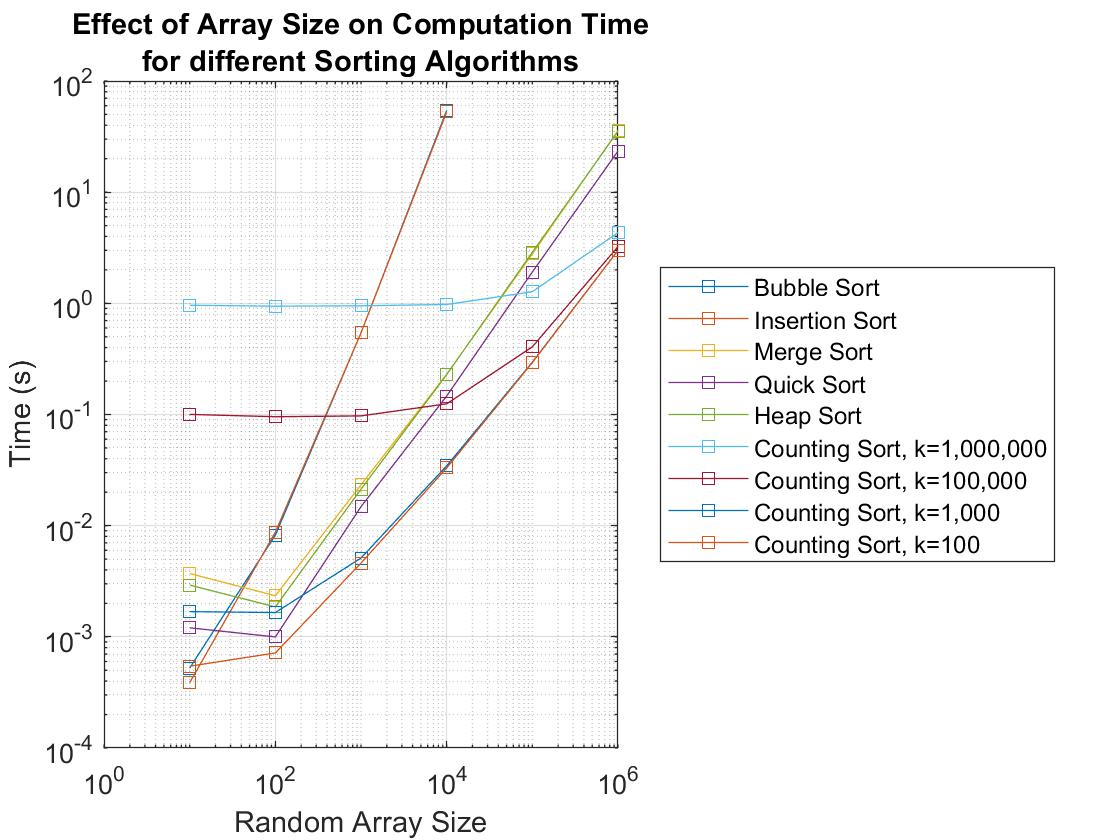
\includegraphics[scale=0.4]{SortTimes}

To gather timing information for several of the presented algorithms, a function is made which takes in a MATLAB sorting algorithm implementation and tests the sorting algorithm on input arrays containing random numbers of length $n$ ranging from $10$ to $10^6$ elements. These times are averaged over $10$ executions to ensure quality of results. Bubble and insertion sort take too long if the input array contains $10^6$ elements, so testing on these functions stops at $10^5$ elements. Counting sort requires too much memory when the elements are from the standard range $(0, 2^{53}-1]$, so the random number generator is limited to a range $(0, k]$, with $k$ varying as indicated in the figure when counting sort is evaluated. The code used to do this comparison and create the figure is included in the appendix.

As can be seen from the detailed descriptions of each algorithm, there are trade-offs involved when selecting a sorting algorithm to solve a specific problem. If the sorting algorithm is going to be operating on smaller arrays with fewer than 100 elements, the reduced instructions required to perform Insertion Sort and Bubble Sort generally lead to these being the best choice.

If the input array is randomized and larger than 100 elements, Quick sort is generally a good choice. During testing, Quick Sort consistently outperformed Heap Sort in terms of computation Time. If the data is in some way structured, Quick Sort could lead to very poor performance. In this situation, Heap Sort would likely be a safer alternative, though the input could be tested for Quick Sort performance. 

Merge Sort is generally not recommended due to the larger space complexity but similar time complexity relative to Heap Sort.

Finally, there if the input data to be sorted involves a limited number of possible keys, Counting Sort can be used to improve performance. Counting Sort can swiftly sort through very large array sizes provided the number of possible keys in the input is small relative to the input’s length.

\section{Appendix}
\subsection{Checking if An Array is Sorted}
\begin{lstlisting}
function [truth] = isminsorted(arr)
%ISSORTED checks if an array is sorted
%   checks for least-to-greatest sort pattern in array
%   returns truth of 'array is sorted'
truth = true;

for i = 1:(length(arr)-1)
    if arr(i) > arr(i+1)
        truth = false;
        break;
    end
end

end
\end{lstlisting}

\subsection{Timing Sorting Algorithms}
\begin{lstlisting}
function [times] = getTimes(func, startlen, stoplen, repeat, maxrand)
% GETTIMES Returns a list of times that correspond to how long
%    the algorithm took to run on arrays 
%    of length 10.^[startlen:stoplen]
%
%    These times are averaged over 'repeat' executions.
%
%    Use 'maxrand' to fix the range of random numbers
%        from 1 to maxrand for evaluating Counting Sort.
% 
if nargin < 5
    if nargin < 4
        repeat = 10;
    end
    maxrand = 2^53-1;
end
times = zeros([1, stoplen - startlen+1]);
time = 0;

for i = 1:repeat
    disp(i)
    for n = 10.^[startlen:stoplen]
        arr = int64(randi(maxrand, 1, n));
        if not(maxrand == 2^53-1)
            tic()
            arr = func(arr, maxrand);
            time = toc();
        else
            tic()
            arr = func(arr);
            time = toc();
        end
        if not(isminsorted(arr))
            disp(arr)
            disp('ERROR ARR NOT SORTED')
        end
        times(log10(n)-startlen + 1) = times(log10(n)-startlen + 1) + time/repeat;
    end
end
end
\end{lstlisting}
\subsection{Evaluate and Plot}
\begin{lstlisting}
repeats = 10

% getTimes(@quicksort, 1, 2000)
times = getTimes(@bubblesort, 1, 4, repeats)
loglog(10.^[1:length(times)], times, '-s', 'DisplayName', 'Bubble Sort')
hold('on')

times = getTimes(@insertionsort, 1, 4, repeats)
loglog(10.^[1:length(times)], times, '-s', 'DisplayName', 'Insertion Sort')

times = getTimes(@mergesort, 1, 6, repeats)
loglog(10.^[1:length(times)], times, '-s', 'DisplayName', 'Merge Sort')

times = getTimes(@quicksort, 1, 6, repeats)
loglog(10.^[1:length(times)], times,'-s', 'DisplayName', 'Quick Sort')

times = getTimes(@heapsort, 1, 6, repeats)
loglog(10.^[1:length(times)], times,'-s', 'DisplayName', 'Heap Sort')

times = getTimes(@countingsort, 1, 6, repeats, 1000000)
loglog(10.^[1:length(times)], times,'-s', 'DisplayName', 'Counting Sort, k=1,000,000')

times = getTimes(@countingsort, 1, 6, repeats, 100000)
loglog(10.^[1:length(times)], times,'-s', 'DisplayName', 'Counting Sort, k=100,000')

times = getTimes(@countingsort, 1, 6, repeats, 1000)
loglog(10.^[1:length(times)], times,'-s', 'DisplayName', 'Counting Sort, k=1,000')

times = getTimes(@countingsort, 1, 6, repeats, 100)
loglog(10.^[1:length(times)], times,'-s', 'DisplayName', 'Counting Sort, k=100')

xlabel('Random Array Size')
ylabel('Time (s)')
legend('location','eastoutside')
title({'Effect of Array Size on Computation Time', 'for different Sorting Algorithms'})
grid('on')

\end{lstlisting}

\end{document}